% aspectration can be 1610, 149, 54, 43 and 32
\documentclass[aspectratio=43,handout]{beamer}

%\setbeameroption{show notes}
\setbeameroption{show only notes}
%\setbeameroption{show notes on second screen=right}

\usefonttheme[onlymath]{serif}
\usepackage{COMP4420_ProjectPresentationStyle}



%****************************************************************************
% DUBUGIN TIPS
%****************************************************************************
% This is used to trace down (pin point) problems
% in latexing a document:
% \tracingall
%****************************************************************************
%****************************************************************************
%****************************************************************************
% The end of the definitions for the document
% The start of the actual document
%****************************************************************************
%****************************************************************************
\begin{document}
	%\pagenumbering{roman}
	
	

\part{Main Presentation}
	%****************************************************************************
	% Title Stuff
	%****************************************************************************
	%\frame{\titlepage}
	\begin{frame}
		\titlepage
	\end{frame}

	%****************************************************************************
	% Begin actual document content here
	%****************************************************************************

	\section{Quicksorts}
		\begin{frame}
			\frametitle{Introduction}
			\begin{itemize}
				\item<+-> $O(n \log(n))$ Average Case Run Time
				\item<+-> In place algorithm
				\item<+-> Pick Pivots
				\item<+-> Partitioning Data
				\item<+-> Recurse to a smaller sub-array
				\item<+-> Use Insertion Sort for a small sub-array
			\end{itemize}
			\note{
				Data is partitioned By Comparing and Swapping elements.
				These will be our metrics.
			}
		\end{frame}	

		\subsection{Classic Quicksort}
			\begin{frame}
				\frametitle{Classic Quicksort}
				\begin{itemize}
					\item<+-> $2n \log n - 1.51n  + O(\log(n))$ Comparisons
					\item<+-> $0.33n \log n - 0.58n + O(\log(n))$ Swaps
					\item<+-> One Pivot
					\begin{itemize}
						\item<+-> First Element
						\item<+-> Last Element
						\item<+-> Median of Three
					\end{itemize}
					\item<+-> Simple Partitioning
					\item<+-> Two Recursive Calls
				\end{itemize}
			\phantom{ }\cite{Wild:2012:ACA:2404160.2404231}
			\end{frame}
		
		\subsection{Dual Pivot Quicksort}
			\begin{frame}
				\frametitle{Dual Pivot Quicksort}
				\begin{itemize}
					\item<+-> $2.13n \log n - 2.57n + O(\log(n))$ Comparisons
					\item<+-> $0.8n \log n -0.3n + O(\log(n))$ Swaps
					\item<+-> Two Pivots
					\begin{itemize}
						\item<+-> First and Last Element
						\item<+-> Middle 2 of 5 elements (Evenly Spaced Out)
					\end{itemize}
					\item<+-> Partitions Smalls then Bigs (Middle is automatic)
					\item<+-> Three Recursive Calls
				\end{itemize}
				\phantom{ }\cite{Wild:2012:ACA:2404160.2404231}
				\note{
					Tertile Elements = Middle 2 of 5 elements (Evenly Spaced Out)
				}
			\end{frame}

			\begin{frame}
				\frametitle{Dual Pivot Quicksort with Optimal Partitioning}
				\begin{itemize}
					\item<+-> $1.8n \log n + O(n)$ Comparisons
					\item<+-> $0.33n \log n + O(n)$ Swaps
					\item<+-> Two Pivots
					\begin{itemize}
						\item<+-> Keeps Tracks of smalls and bigs
						\item<+-> Uses the information to see who to compare to first
					\end{itemize}
					\item<+-> Otherwise very similar to standard Dual Pivot Quicksort
				\end{itemize}
				\phantom{ }\cite{Aumuller:2013:OPD:2525857.2525862}
			\end{frame}


		\subsection{Yaroslavskiy's Quicksort}
			\begin{frame}
				\frametitle{Yaroslavskiy's Dual Pivot Quicksort}
				\begin{itemize}
					\item<+-> $1.9n \log n - 2.46n + O(\log(n)$ Comparisons
					\item<+-> $0.6n \log n + 0.08n + O(\log(n))$ Swaps
					\item<+-> Two Pivots
					\begin{itemize}
						\item<+-> Middle 2 of 5 elements (Evenly Spaced Out)
						\item<+-> Uses 5-element sorting network
					\end{itemize}
					\item<+-> Simultaneous Partition algorithm
					\item<+-> Two Recursive Calls 
				\end{itemize}
				\phantom{ }\cite{Wild:2012:ACA:2404160.2404231}
				\note{
					It turns out that Yaroslavskiy’s partitioning method is able to 
					take advantage of certain asymmetries in the outcomes of key comparisons.
					While the Regular Dual Pivot quicksort fails to utilize them, even though
					being based on the same abstract algorithmic idea.
				}
			\end{frame}

		\subsection{Three Pivot Quicksort}
			\begin{frame}
				\frametitle{Kushagra-Ortiz-Qiao-Munro Tri-Pivot Quicksort}
				\begin{itemize}
					\item<+-> $1.846n \log n + O(n)$ Comparisons
					\item<+-> $0.615n \log n + O(n)$ Swaps
					\item<+-> Three Pivots
					\begin{itemize}
						\item<+-> Middle 3 of 7 elements (Evenly Spaced Out)
					\end{itemize}
					\item<+-> Simultaneous Partition algorithm
					\item<+-> Four Recursive Calls 
				\end{itemize}
				\phantom{ }\cite{kushagra2013multi}
				\note{
					This algorithm had incomplete pseudo-code.
					Only the partition algorithm was specified.
					Later on we see that this algorithm doesn't do well.
					It may be due to some choices we made in our implementation.
				}
			\end{frame}
		
		\subsection{M-Pivot Quicksort}
			\begin{frame}
				\frametitle{M-Pivot Quicksort}
				\begin{itemize}
					\item<+-> $O(n \log n)$ Comparisons
					\item<+-> $O(n \log n)$ Swaps
					\item<+-> $M$ Pivots
					\begin{itemize}
						\item<+-> Sort $2M$ elements then pick ever other element
					\end{itemize}
					\item<+-> Partition each segment one at a time 
					\item<+-> $M+1$ Recursive Calls
				\end{itemize}
				\phantom{ }\cite{edmondson2007multiple}
				\note{
					The run times discussed thus far have been for specific pivots.
					The analysis for each pivot and how one partition changes the analysis,
					which depends on studying the decision tree generated.
				}
			\end{frame}
		
			\begin{frame}
				\frametitle{Example M-Pivot Selection and Partitioning}
				\begin{center}   
					\includegraphics<1>[width=70mm]{MPivotSelectCanadates.png}
					\includegraphics<2>[width=72mm]{MPivotSelection.png}
					\includegraphics<3>[width=72mm]{MPivotPartiton.png}
				\end{center}

				\phantom{ }\cite{edmondson2007multiple}
			\end{frame}

			\begin{frame}
				\begin{itemize}
					\frametitle{Heap Optimized M-Pivot Quicksort}
					\item<+-> Enforce the Heap Property to the array before any computation
					\begin{itemize}
						\item<+-> Adds only $O(n)$ run time at each call
						\item<+-> Improves the sort to optimize pivot selection
					\end{itemize}
				\end{itemize}
				\phantom{ }\cite{edmondson2007multiple}
			\end{frame}

			\begin{frame}
				\frametitle{Example M-Pivot Heap Optimized Pivot Selection}
				\begin{center}   
					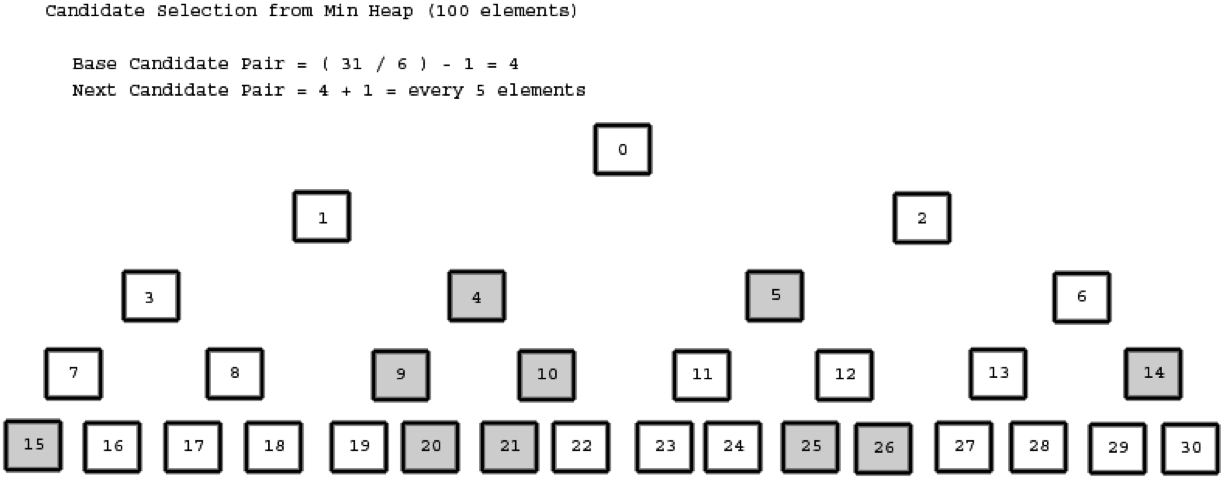
\includegraphics[width=97mm]{MPivotHeap.png}
				\end{center}
				\phantom{ }\cite{edmondson2007multiple}
			\end{frame}

		\subsection{Summary}
			\begin{frame}
				\frametitle{Theoretical Average Case Run Time}
				\only<1>{
					\begin{center}
						\begin{tabular}{|r|l|}
							\hline
							Sort Method        &   Comparisons                          \\ \hline \hline
							Classic            &   $2n \log n - 1.51n  + O(\log(n))$   \\ \hline
							Dual Pivot         &   $2.13n \log n - 2.57n + O(\log(n))$ \\ \hline
							Optimal Dual Pivot &   $1.8n \log n + O(n)$               \\ \hline
							Three Pivot        &   $1.846n \log n + O(n)$             \\ \hline
							Yaroslavskiy       &   $1.9n \log n - 2.46n + O(\log(n)$  \\ \hline
							M Pivot            &   $O(n \log n)$                        \\ 
							\hline
						\end{tabular}
					\end{center}
				}
				\only<2>{
					\begin{center}
						\begin{tabular}{|r|l|}
							\hline
							Sort Method         &     Swaps \\ \hline \hline
							Classic             &  $0.33n \log n - 0.58n + O(\log(n))$\\ \hline
							Dual Pivot          &  $0.8n \log n -0.3n + O(\log(n))$   \\ \hline
							Optimal Dual Pivot  &  $0.33n \log n + O(n)$              \\ \hline
							Three Pivot         &  $0.615n \log n + O(n)$             \\ \hline
							Yaroslavskiy        &  $0.6n \log n + 0.08n + O(\log(n))$  \\ \hline
							M Pivot             &  $O(n \log n)$ \\ 
							\hline
						\end{tabular}
					\end{center}				
				}
				\phantom{ }\cite{Aumuller:2013:OPD:2525857.2525862}\\
				\phantom{ }\cite{Wild:2012:ACA:2404160.2404231}\\
				\phantom{ }\cite{kushagra2013multi}
				\note{
					These are average case run times.
					The M-Pivot quicksort is not studied very well.
					As you see, people study each quicksort with a fixed number of pivots.
				}
			\end{frame}


	\section{Legend}
		\begin{frame}
			\frametitle{Legend}
			\begin{center}   
				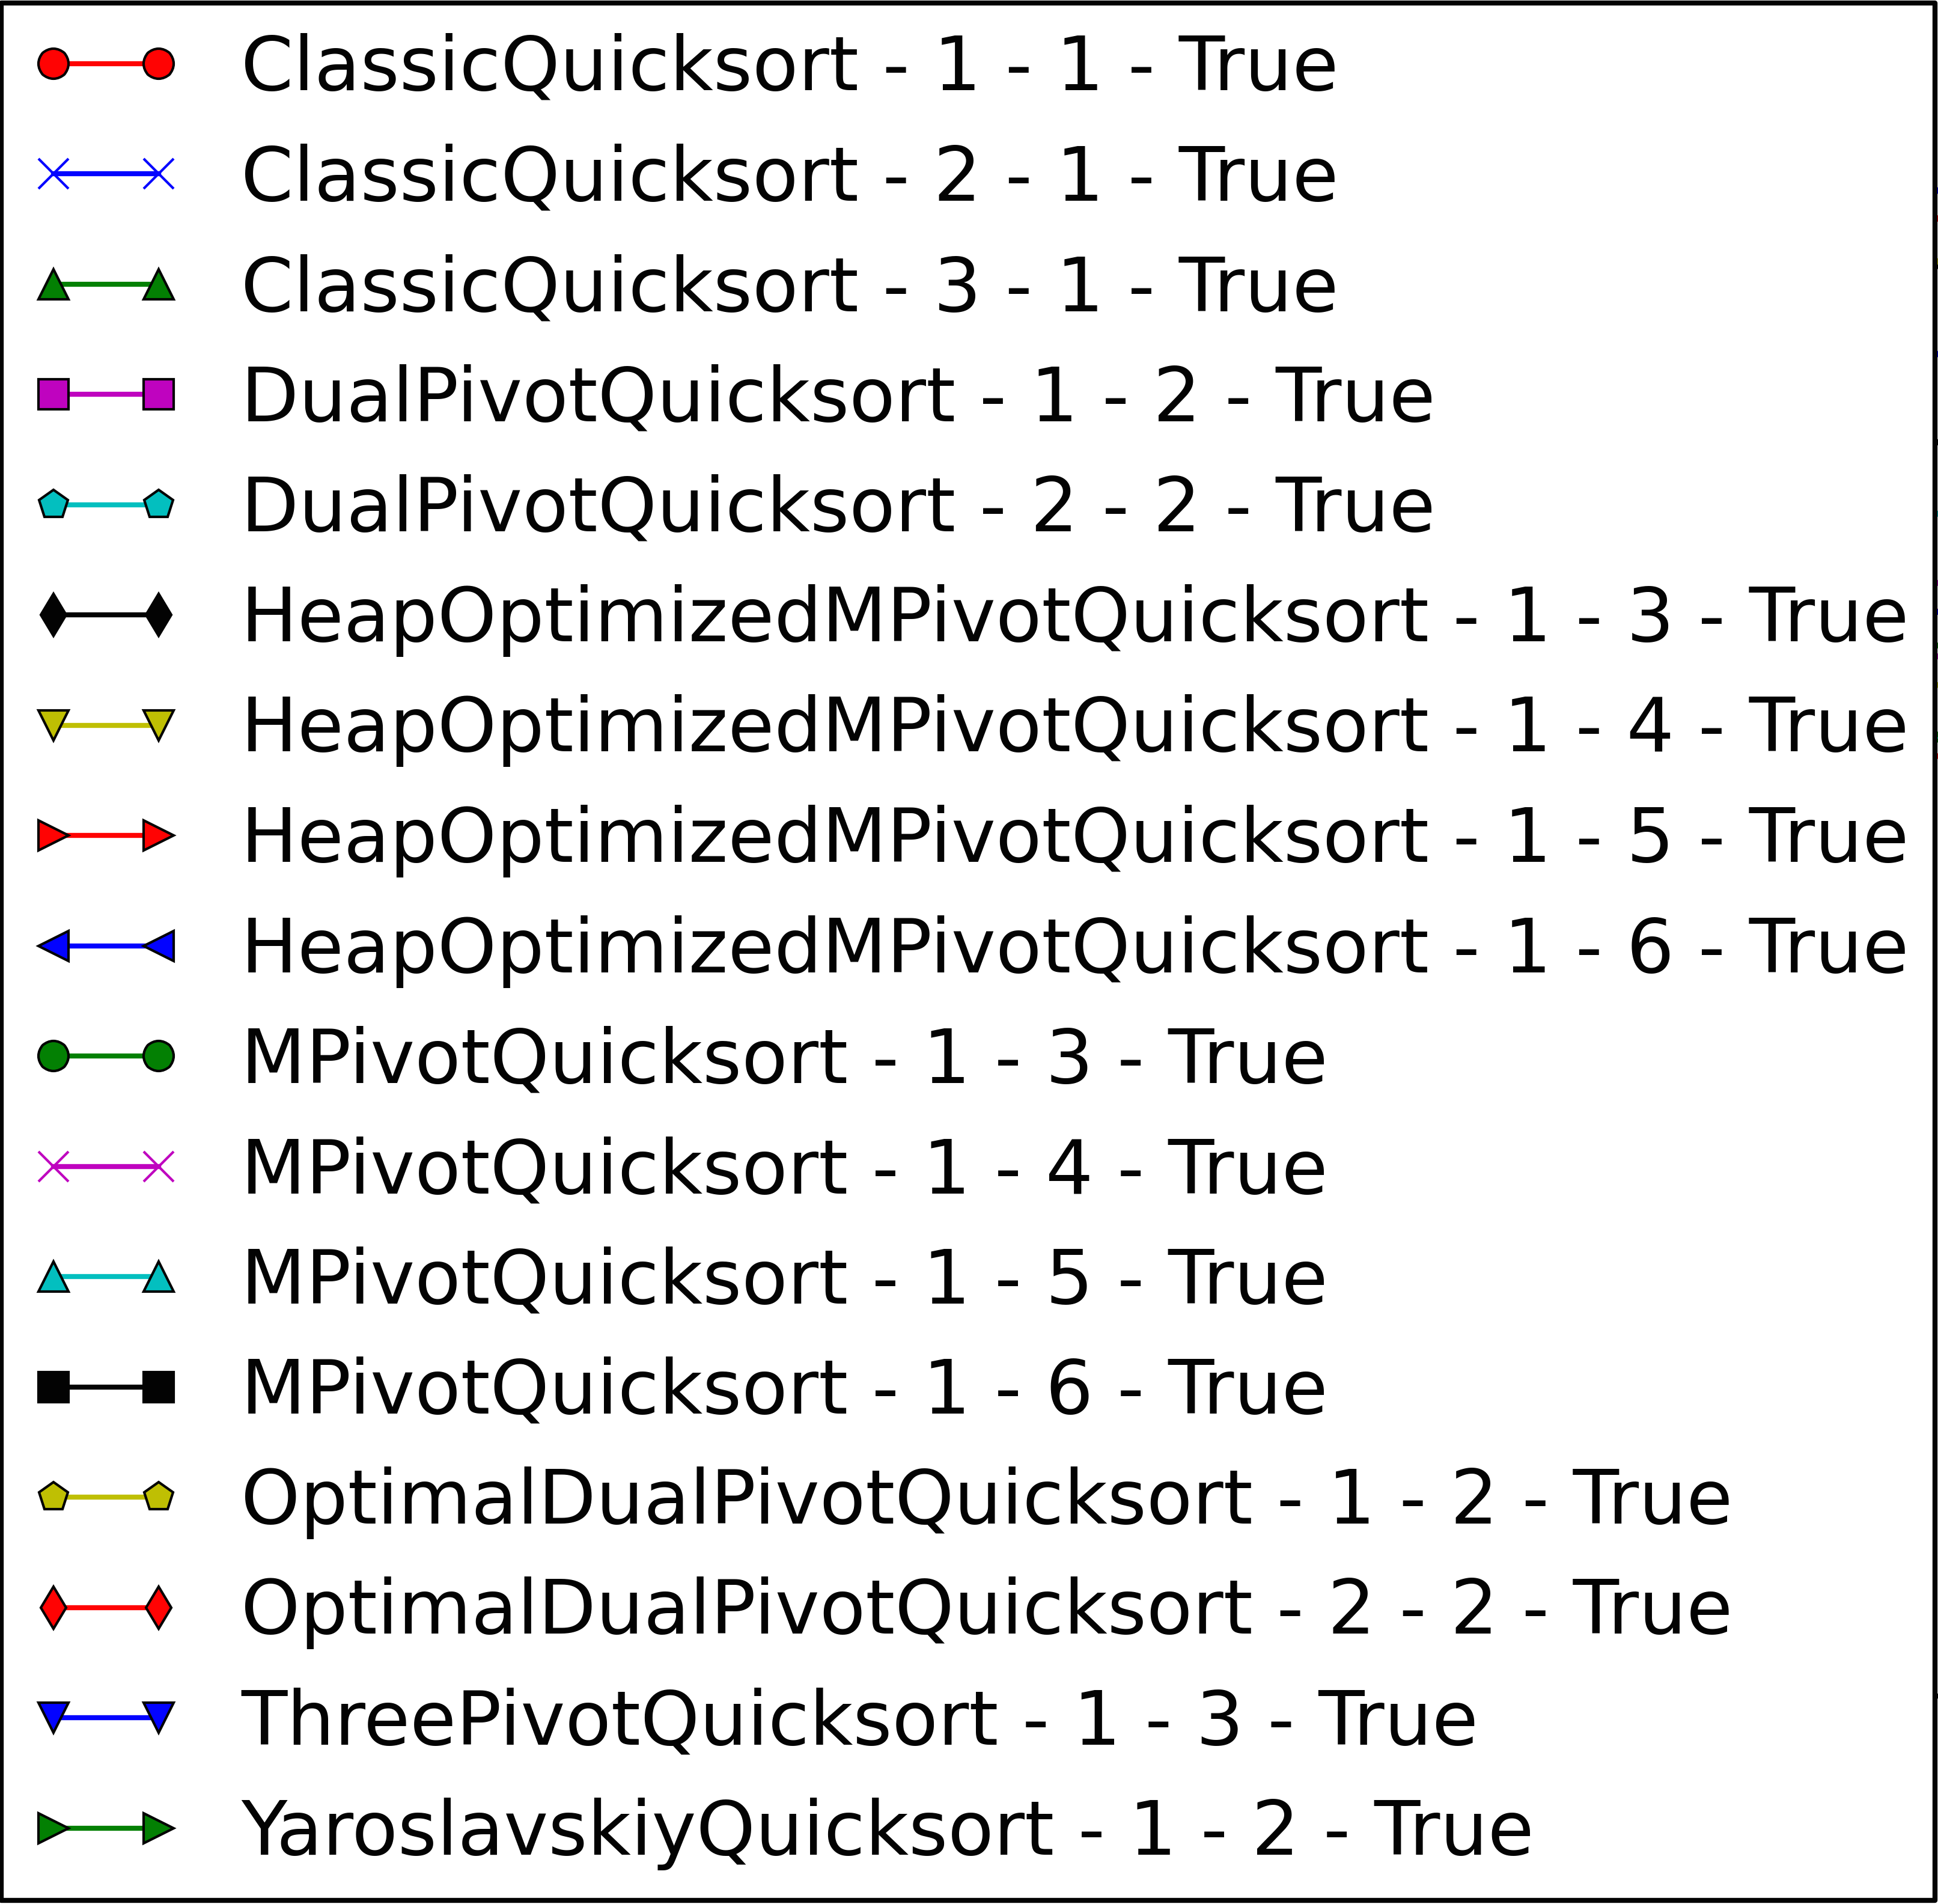
\includegraphics[width=72mm]{PlotLegend.png}
				\label{fig:PlotLegend}
			\end{center}
		\note{
			You can see the color and shape combination for each version of
			quick sort. These color and shape choices will be consistent throughout
			the following plots.
			There are 17 distinct derivatives of quicksort that have been run.

			Note that for the large scale plot. We overlay the function :\\
				$A\cdot n\log(n) + B\cdot n + C \log(n)$ \\
			With the function parameters $A,B$ and $C$ where found using a
			curve fitter on the data.
			As you will see in the following plots. The function are 'good ' fits.
			We have not done analysis to see if we have over fit our data.
			Although from the analysis done in many of the papers, the functions
			have that form. \\
			Also for the small scale plots. The curve fitted function may not be
			seen, as a result, we just connect the data points and only show the
			fitted curve in the large scale plots.
		}
		\end{frame}

	\section{Results}
		\subsection{Mass Comparison}
			\begin{frame}
				\frametitle{Mass Comparison Small Scale}
				\begin{center}   
					\includegraphics<1>[width=97mm]{AllthePlotsSmallScale_comp.png}
					\includegraphics<2>[width=97mm]{AllthePlotsSmallScale_swap.png}
				\end{center}
				
				\note{
					Comparisons :

					The Heap 6-pivot sort is the worst. 
					Close with all the other heap m-pivot sorts. 
					5-Pivot sort, 4-pivot sort, 3-pivot sort and Three-pivot quicksort
					all seem to be mediocre.
					The classic quicksorts, yaro, dual pivot, and optimal dual pivot 
					all seem to be close and doing well

					Swaps :

					Similar trend as comparisons.
					Although the classic quicksorts are much higher than expected.
					They are close to the heap m-pivot sorts.
				}
			\end{frame}

			\begin{frame}
				\frametitle{Mass Comparison Large Scale}

				\begin{center}   
					\includegraphics<1>[width=97mm]{AllthePlotsLargeScale_comp.png}
					\includegraphics<2>[width=97mm]{AllthePlotsLargeScale_swap.png}
				\end{center}
				\note{
					Comparisons :
						Optimized dual pivot quicksort, yaro, M-pivot sorts do well
						Heap Optimized m-pivot sorts do badly
					Swaps :
						Heap Optimized Sorts still do badly relative to the rest.
						Classic quicksorts also doing badly.
				}
			\end{frame}

			\begin{frame}
				\frametitle{Mass Comparison $\log(n)$ vs $\frac{y}{n \log(n)}$}

				\begin{center}   
					\includegraphics<1>[width=97mm]{AllPlotsLargeScalelognvsy_OVER_nlogn_comp.png}
					\includegraphics<2>[width=97mm]{AllPlotsLargeScalelognvsy_OVER_nlogn_swap.png}
				\end{center}
				\note{
					The point of these two plots is to emphasize the trend we see.
					In the last figure, all the plots look linear-like and doing
					it's own thing. In this plot there is a clear fact that all the
					plots have a trend.

					Comparisons :

					Swaps :
				}
			\end{frame}


		\subsection{One Pivot}
			\begin{frame}
				\frametitle{One Pivot Comparison Small Scale}

				\begin{center}   
					\includegraphics<1>[width=97mm]{OnePivotsSmallScale_comp.png}
					\includegraphics<2>[width=97mm]{OnePivotsSmallScale_swap.png}
				\end{center}
				\note{
					Comparisons :

					Swaps :

				}
			\end{frame}

			\begin{frame}
				\frametitle{One Pivot Comparison Large Scale}

				\begin{center}   
					\includegraphics<1>[width=97mm]{OnePivotsLargeScale_comp.png}
					\includegraphics<2>[width=97mm]{OnePivotsLargeScale_swap.png}
				\end{center}
				\note{
					Comparisons :

					Swaps :

				}
			\end{frame}


		\subsection{Two Pivots}
			\begin{frame}
				\frametitle{Two Pivot Comparison Small Scale}

				\begin{center}   
					\includegraphics<1>[width=97mm]{TwoPivotsSmallScale_comp.png}
					\includegraphics<2>[width=97mm]{TwoPivotsSmallScale_swap.png}
				\end{center}
				\note{
					Comparisons :
						They are all doing very similarly.
					Swaps :
						Optimal Dual Pivot quicksort and dual pivot quicksort are doing really well.
						Yaro isn't.
				}
			\end{frame}

			\begin{frame}
				\frametitle{Two Pivot Comparison Large Scale}

				\begin{center}   
					\includegraphics<1>[width=97mm]{TwoPivotsLargeScale_comp.png}
					\includegraphics<2>[width=97mm]{TwoPivotsLargeScale_swap.png}
				\end{center}
				\note{
					Comparisons :
						We can start to see them split.
						Optimal Dual Pivot Quicksort [second option] still rocks.
						Dual Picot [1] and Optimal Dual Pivot [1] don't do well.
					Swaps :
						They all do very similarly.
						Optimal Dual [1] and Dual Pivot [1] start to split away.
				}
			\end{frame}

		\subsection{Three Pivots}
			\begin{frame}
				\frametitle{Three Pivot Comparison Small Scale}
				\begin{center}   
					\includegraphics<1>[width=97mm]{ThreePivotsSmallScale_comp.png}
					\includegraphics<2>[width=97mm]{ThreePivotsSmallScale_swap.png}
				\end{center}
				\note{
					Comparisons :
						Interpertations Clear From plot.
						3-Pivot Sort is great then the Three-pivot-Quicksort
					Swaps :
						Three-pivot-Quicksort is great then the 3-Pivot Sort

					In both cases heap 3-pivot sort is the worst.
				}
			\end{frame}

			\begin{frame}
				\frametitle{Three Pivot Comparison Large Scale}
				\begin{center}   
					\includegraphics<1>[width=97mm]{ThreePivotsLargeScale_comp.png}
					\includegraphics<2>[width=97mm]{ThreePivotsLargeScale_swap.png}	
				\end{center}
				\note{
					Comparisons :
						Same as the small scale
					Swaps :
						Same as the small scale
				}
			\end{frame}

		\subsection{M Pivots}
			\begin{frame}
				\frametitle{M Pivot Comparison Small Scale}
				\begin{center}   
					\includegraphics<1>[width=97mm]{M-PivotQuicksortsSmallScale_comp.png}
					\includegraphics<2>[width=97mm]{M-PivotQuicksortsSmallScale_swap.png}
				\end{center}
				\note{
					Comparisons :
						3-pivot sort rocks.
						Heap 6-pivot sort sucks.
					Swaps :
						3,4,5-pivot sort are really good.
						Heap 3-pivot sort is bad.
				}
			\end{frame}

			\begin{frame}
				\frametitle{M Pivot Comparison Large Scale}
				\begin{center}   
					\includegraphics<1>[width=97mm]{M-PivotQuicksortsLargeScale_comp.png}
					\includegraphics<2>[width=97mm]{M-PivotQuicksortsLargeScale_swap.png}
				\end{center}
				\note{
					Comparisons :
						3,4,5-pivot sort are really good.
						All the heap-m-pivot sorts are not
					Swaps :
						6-pivot sort is the best.
						Although 3,4,5-pivot sorts are good as well.
						All the heap-m-pivot sorts are not good.
				}
			\end{frame}


		\subsection{Curve Fit}
			\begin{frame}
				\frametitle{Fit Coefficients of $A\cdot n\log(n) + B\cdot n + C \log(n)$ }
				\only<1>{
					\begin{center}
						\begin{tabular}{|r|c|c|}
							\hline
							               Sort Method & Comparisons         &   Swaps             \\ \hline \hline
						               Classic - 1 - 1 &   0.02219           &   0.01060           \\ \hline
						               Classic - 2 - 1 &   0.02126           & {\bfseries 0.01110} \\ \hline
						               Classic - 3 - 1 &   0.01799           &   0.00828           \\ \hline
						            Dual Pivot - 1 - 2 &   0.02109           &   0.00636           \\ \hline
						            Dual Pivot - 2 - 2 &   0.01787           &   0.00603           \\ \hline
						    Optimal Dual Pivot - 1 - 2 &   0.02044           &   0.00636           \\ \hline
						    Optimal Dual Pivot - 2 - 2 & {\bfseries 0.01754} &   0.00603           \\ \hline
						           Three Pivot - 1 - 3 &   0.02595           &   0.00616           \\ \hline
						          Yaroslavskiy - 1 - 2 &   0.01811           &   0.00584           \\ \hline
						\end{tabular}
					\end{center}
				}
				\only<2>{
					\begin{center}
						\begin{tabular}{|r|c|c|}
							\hline
							               Sort Method & Comparisons         &   Swaps             \\ \hline \hline
						          Heap M Pivot - 1 - 3 &   0.02755           &   0.00999           \\ \hline
						          Heap M Pivot - 1 - 4 &   0.02782           &   0.00885           \\ \hline
						          Heap M Pivot - 1 - 5 & {\bfseries 0.02903} &   0.00809           \\ \hline
						          Heap M Pivot - 1 - 6 &   0.02801           &   0.00769           \\ \hline
						               M Pivot - 1 - 3 &   0.01955           &   0.00640           \\ \hline
						               M Pivot - 1 - 4 &   0.02039           &   0.00594           \\ \hline
						               M Pivot - 1 - 5 &   0.02136           &   0.00532           \\ \hline
						               M Pivot - 1 - 6 &   0.02369           & {\bfseries 0.00524} \\ \hline
						\end{tabular}
					\end{center}			
				}
				\note{
					Name of sort - Pivot Selection Method - Number of Pivots

					The values in the table are of the coefficient of the $n\log(n)$ term.
					\\
					Best Comparisons  : Optimal Dual Pivot - 2 - 2 \\
					Best Swaps        : M Pivot - 1 - 6            \\
					Worst Comparisons : Heap M Pivot - 1 - 5       \\
					Worst Swaps       : Classic - 2 - 1            \\
					\\
					Overall we see that the Heap-M-Pivot sort do terribly.
					This may be a result of how often we call Heapify.
					We may have not needed to call heapify at every recursive call.
					This can be an error on our part.
				}
			\end{frame}


	\section{The End}

		%****************************************************************************
		% Reference frames/slides
		%****************************************************************************
		\begin{frame}[allowframebreaks]
			\frametitle{References}    
			\bibliographystyle{plainnat}
			\bibliography{../References/refer}
		\end{frame}

		\begin{frame}
			\begin{center}
				\Huge Questions?
			\end{center}
		\end{frame}

\part{Answers}
	\begin{frame}
		% Empty Frame
		\note{
			Will add slides to answer potential questions.
		}
	\end{frame}


	\begin{frame}
		% Empty Frame
		\note{
			
		}
	\end{frame}

%****************************************************************************
% End of the contents of the document
% Items related to end of document
%****************************************************************************
\end{document}